\chapter{Implementation}\label{ch:implementation}

% Implementation details

The first step is to implement the state-of-the-art in image regeneration to guage the improvements. We use DCGAN to start of with. The results of the training and testing will be recorded to compare it with the results of our CapsNet-based approach later. We will be using CapsNet as the underlying technology to implement our GAN (CapsGAN). The goal is to replace the CNN inside DCGAN with CapsNet and compare the results. The GAN internally consists of two components - a generator and a discriminator - which we build out of CapsNet. The discriminator is initially trained separately to distinguish real and fake data, and later they work together to improve upon their performance by acting as adversaries.
\par\bigskip

\begin{figure}[H]
\centering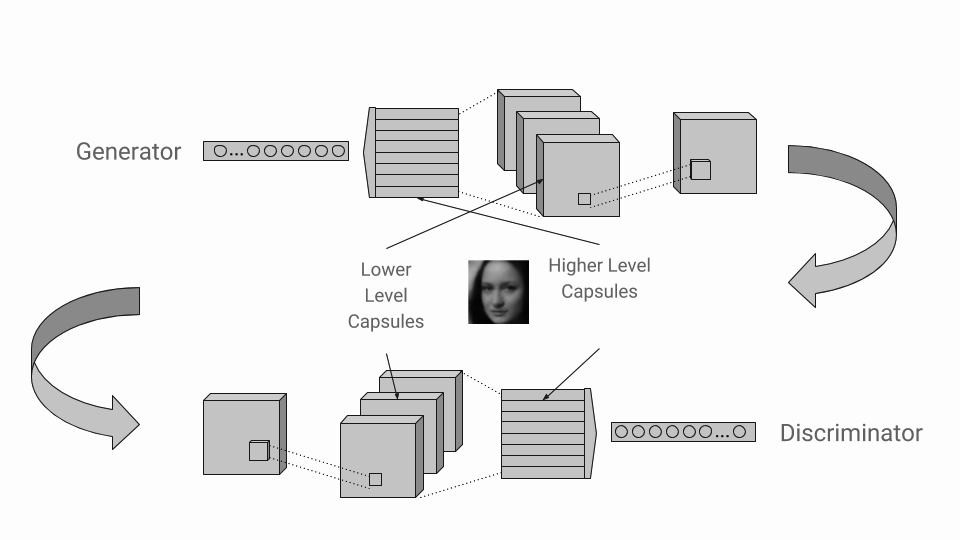
\includegraphics[width=1\textwidth]{images/methodology.png}
\caption{Proposed architecture}
\label{fig:capsgan}
\end{figure}

During the course of our research we were forced to conclude that building a CapsNet based generator was not feasible. A fundamental aspect of a GAN is back-propagation in the discriminator which is not possible to replicate in the generator. Hence we implemented just the discriminator in CapsNet. 
\par\bigskip

We concentrated on four networks: DCGAN, WGAN, ACGAN and InfoGAN. Our training laboratory was Colloboratory - the cloud machine learning research platform. We trained each network individually for 20,000 epochs each. For our preliminary training we used the MNIST dataset. The MNIST dataset is a large dataset of handwritten digits commonly used for image processing training tasks. Each of the networks had it's discriminator augmented with the CapsNet code. The networks with the CapsNet discriminator were then individually trained on the same dataset, for 20,000 epochs each. Overall, it took us a few days to train all the networks and gather all the data.
\par\bigskip

\section{Network Architectures} % (fold)
\label{sec:network_architectures}
The following are the network architectures of the generator and the discriminator.

\subsection{Generator} % (fold)
\label{sub:generator}
\begin{lstlisting}[basicstyle=\scriptsize,language=Python]
_________________________________________________________________
Layer (type)                 Output Shape              Param #   
=================================================================
dense_5 (Dense)              (None, 8192)              827392    
_________________________________________________________________
reshape_1 (Reshape)          (None, 8, 8, 128)         0         
_________________________________________________________________
batch_normalization_3 (Batch (None, 8, 8, 128)         512       
_________________________________________________________________
up_sampling2d_1 (UpSampling2 (None, 16, 16, 128)       0         
_________________________________________________________________
conv2d_1 (Conv2D)            (None, 16, 16, 128)       147584    
_________________________________________________________________
activation_1 (Activation)    (None, 16, 16, 128)       0         
_________________________________________________________________
batch_normalization_4 (Batch (None, 16, 16, 128)       512       
_________________________________________________________________
up_sampling2d_2 (UpSampling2 (None, 32, 32, 128)       0         
_________________________________________________________________
conv2d_2 (Conv2D)            (None, 32, 32, 64)        73792     
_________________________________________________________________
activation_2 (Activation)    (None, 32, 32, 64)        0         
_________________________________________________________________
batch_normalization_5 (Batch (None, 32, 32, 64)        256       
_________________________________________________________________
up_sampling2d_3 (UpSampling2 (None, 64, 64, 64)        0         
_________________________________________________________________
conv2d_3 (Conv2D)            (None, 64, 64, 32)        18464     
_________________________________________________________________
activation_3 (Activation)    (None, 64, 64, 32)        0         
_________________________________________________________________
batch_normalization_6 (Batch (None, 64, 64, 32)        128       
_________________________________________________________________
conv2d_4 (Conv2D)            (None, 64, 64, 3)         867       
_________________________________________________________________
activation_4 (Activation)    (None, 64, 64, 3)         0         
=================================================================
Total params: 1,069,507
Trainable params: 1,068,803
Non-trainable params: 704
_________________________________________________________________
\end{lstlisting}
% subsection generator (end)

\subsection{Discriminator} % (fold)
\label{sub:discriminator}
\begin{lstlisting}[basicstyle=\scriptsize,language=Python]
__________________________________________________________________________________________________
Layer (type)                    Output Shape         Param #     Connected to                     
==================================================================================================
input_1 (InputLayer)            (None, 64, 64, 3)    0                                            
__________________________________________________________________________________________________
conv1 (Conv2D)                  (None, 56, 56, 256)  62464       input_1[0][0]                    
__________________________________________________________________________________________________
leaky_re_lu_1 (LeakyReLU)       (None, 56, 56, 256)  0           conv1[0][0]                      
__________________________________________________________________________________________________
batch_normalization_1 (BatchNor (None, 56, 56, 256)  1024        leaky_re_lu_1[0][0]              
__________________________________________________________________________________________________
primarycap_conv2 (Conv2D)       (None, 24, 24, 256)  5308672     batch_normalization_1[0][0]      
__________________________________________________________________________________________________
primarycap_reshape (Reshape)    (None, 18432, 8)     0           primarycap_conv2[0][0]           
__________________________________________________________________________________________________
primarycap_squash (Lambda)      (None, 18432, 8)     0           primarycap_reshape[0][0]         
__________________________________________________________________________________________________
batch_normalization_2 (BatchNor (None, 18432, 8)     32          primarycap_squash[0][0]          
__________________________________________________________________________________________________
flatten_1 (Flatten)             (None, 147456)       0           batch_normalization_2[0][0]      
__________________________________________________________________________________________________
uhat_digitcaps (Dense)          (None, 160)          23593120    flatten_1[0][0]                  
__________________________________________________________________________________________________
softmax_digitcaps1 (Activation) (None, 160)          0           uhat_digitcaps[0][0]             
__________________________________________________________________________________________________
dense_1 (Dense)                 (None, 160)          25760       softmax_digitcaps1[0][0]         
__________________________________________________________________________________________________
multiply_1 (Multiply)           (None, 160)          0           uhat_digitcaps[0][0]             
                                                                 dense_1[0][0]                    
__________________________________________________________________________________________________
leaky_re_lu_2 (LeakyReLU)       (None, 160)          0           multiply_1[0][0]                 
__________________________________________________________________________________________________
softmax_digitcaps2 (Activation) (None, 160)          0           leaky_re_lu_2[0][0]              
__________________________________________________________________________________________________
dense_2 (Dense)                 (None, 160)          25760       softmax_digitcaps2[0][0]         
__________________________________________________________________________________________________
multiply_2 (Multiply)           (None, 160)          0           uhat_digitcaps[0][0]             
                                                                 dense_2[0][0]                    
__________________________________________________________________________________________________
leaky_re_lu_3 (LeakyReLU)       (None, 160)          0           multiply_2[0][0]                 
__________________________________________________________________________________________________
softmax_digitcaps3 (Activation) (None, 160)          0           leaky_re_lu_3[0][0]              
__________________________________________________________________________________________________
dense_3 (Dense)                 (None, 160)          25760       softmax_digitcaps3[0][0]         
__________________________________________________________________________________________________
multiply_3 (Multiply)           (None, 160)          0           uhat_digitcaps[0][0]             
                                                                 dense_3[0][0]                    
__________________________________________________________________________________________________
leaky_re_lu_4 (LeakyReLU)       (None, 160)          0           multiply_3[0][0]                 
__________________________________________________________________________________________________
dense_4 (Dense)                 (None, 1)            161         leaky_re_lu_4[0][0]              
==================================================================================================
Total params: 29,042,753
Trainable params: 29,042,225
Non-trainable params: 528
__________________________________________________________________________________________________
\end{lstlisting}
% subsection discriminator (end)

% section network_architectures (end)













% \begin{figure}[H]
% \centering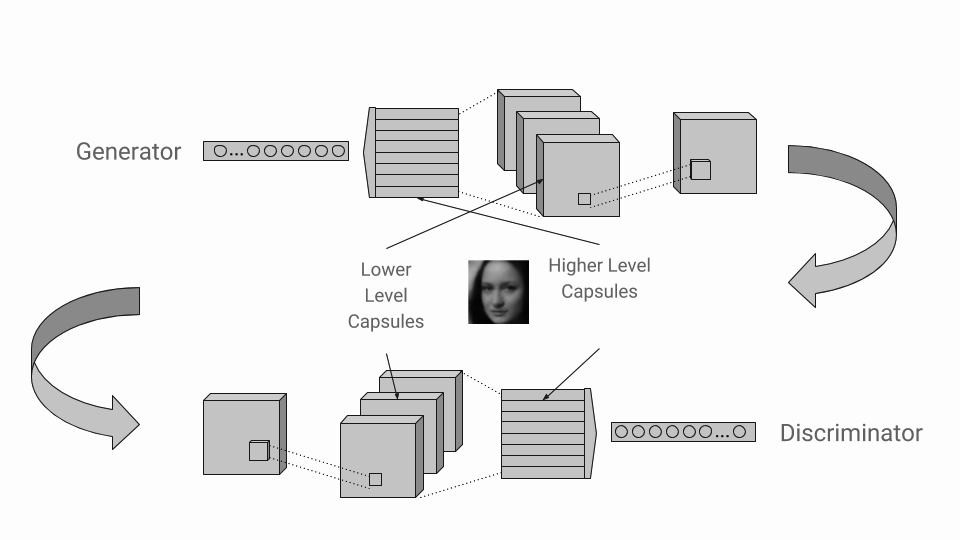
\includegraphics[width=1\textwidth]{images/methodology.png}
% \caption{Proposed architecture}
% \label{fig:capsgan}
% \end{figure}



% _________________________________________________________________
% Layer (type)                 Output Shape              Param #   
% =================================================================
% dense_5 (Dense)              (None, 8192)              827392    
% _________________________________________________________________
% reshape_1 (Reshape)          (None, 8, 8, 128)         0         
% _________________________________________________________________
% batch_normalization_3 (Batch (None, 8, 8, 128)         512       
% _________________________________________________________________
% up_sampling2d_1 (UpSampling2 (None, 16, 16, 128)       0         
% _________________________________________________________________
% conv2d_1 (Conv2D)            (None, 16, 16, 128)       147584    
% _________________________________________________________________
% activation_1 (Activation)    (None, 16, 16, 128)       0         
% _________________________________________________________________
% batch_normalization_4 (Batch (None, 16, 16, 128)       512       
% _________________________________________________________________
% up_sampling2d_2 (UpSampling2 (None, 32, 32, 128)       0         
% _________________________________________________________________
% conv2d_2 (Conv2D)            (None, 32, 32, 64)        73792     
% _________________________________________________________________
% activation_2 (Activation)    (None, 32, 32, 64)        0         
% _________________________________________________________________
% batch_normalization_5 (Batch (None, 32, 32, 64)        256       
% _________________________________________________________________
% up_sampling2d_3 (UpSampling2 (None, 64, 64, 64)        0         
% _________________________________________________________________
% conv2d_3 (Conv2D)            (None, 64, 64, 32)        18464     
% _________________________________________________________________
% activation_3 (Activation)    (None, 64, 64, 32)        0         
% _________________________________________________________________
% batch_normalization_6 (Batch (None, 64, 64, 32)        128       
% _________________________________________________________________
% conv2d_4 (Conv2D)            (None, 64, 64, 3)         867       
% _________________________________________________________________
% activation_4 (Activation)    (None, 64, 64, 3)         0         
% =================================================================
% Total params: 1,069,507
% Trainable params: 1,068,803
% Non-trainable params: 704
% \begin{lstlisting}[basicstyle=\scriptsize,]
% __________________________________________________________________________________________________
% Layer (type)                    Output Shape         Param #     Connected to                     
% ==================================================================================================
% input_1 (InputLayer)            (None, 64, 64, 3)    0                                            
% __________________________________________________________________________________________________
% conv1 (Conv2D)                  (None, 56, 56, 256)  62464       input_1[0][0]                    
% __________________________________________________________________________________________________
% leaky_re_lu_1 (LeakyReLU)       (None, 56, 56, 256)  0           conv1[0][0]                      
% __________________________________________________________________________________________________
% batch_normalization_1 (BatchNor (None, 56, 56, 256)  1024        leaky_re_lu_1[0][0]              
% __________________________________________________________________________________________________
% primarycap_conv2 (Conv2D)       (None, 24, 24, 256)  5308672     batch_normalization_1[0][0]      
% __________________________________________________________________________________________________
% primarycap_reshape (Reshape)    (None, 18432, 8)     0           primarycap_conv2[0][0]           
% __________________________________________________________________________________________________
% primarycap_squash (Lambda)      (None, 18432, 8)     0           primarycap_reshape[0][0]         
% __________________________________________________________________________________________________
% batch_normalization_2 (BatchNor (None, 18432, 8)     32          primarycap_squash[0][0]          
% __________________________________________________________________________________________________
% flatten_1 (Flatten)             (None, 147456)       0           batch_normalization_2[0][0]      
% __________________________________________________________________________________________________
% uhat_digitcaps (Dense)          (None, 160)          23593120    flatten_1[0][0]                  
% __________________________________________________________________________________________________
% softmax_digitcaps1 (Activation) (None, 160)          0           uhat_digitcaps[0][0]             
% __________________________________________________________________________________________________
% dense_1 (Dense)                 (None, 160)          25760       softmax_digitcaps1[0][0]         
% __________________________________________________________________________________________________
% multiply_1 (Multiply)           (None, 160)          0           uhat_digitcaps[0][0]             
%                                                                  dense_1[0][0]                    
% __________________________________________________________________________________________________
% leaky_re_lu_2 (LeakyReLU)       (None, 160)          0           multiply_1[0][0]                 
% __________________________________________________________________________________________________
% softmax_digitcaps2 (Activation) (None, 160)          0           leaky_re_lu_2[0][0]              
% __________________________________________________________________________________________________
% dense_2 (Dense)                 (None, 160)          25760       softmax_digitcaps2[0][0]         
% __________________________________________________________________________________________________
% multiply_2 (Multiply)           (None, 160)          0           uhat_digitcaps[0][0]             
%                                                                  dense_2[0][0]                    
% __________________________________________________________________________________________________
% leaky_re_lu_3 (LeakyReLU)       (None, 160)          0           multiply_2[0][0]                 
% __________________________________________________________________________________________________
% softmax_digitcaps3 (Activation) (None, 160)          0           leaky_re_lu_3[0][0]              
% __________________________________________________________________________________________________
% dense_3 (Dense)                 (None, 160)          25760       softmax_digitcaps3[0][0]         
% __________________________________________________________________________________________________
% multiply_3 (Multiply)           (None, 160)          0           uhat_digitcaps[0][0]             
%                                                                  dense_3[0][0]                    
% __________________________________________________________________________________________________
% leaky_re_lu_4 (LeakyReLU)       (None, 160)          0           multiply_3[0][0]                 
% __________________________________________________________________________________________________
% dense_4 (Dense)                 (None, 1)            161         leaky_re_lu_4[0][0]              
% ==================================================================================================
% Total params: 29,042,753
% Trainable params: 29,042,225
% Non-trainable params: 528
% __________________________________________________________________________________________________
% \end{lstlisting}
